% 注意事项:编译两次,以确保目录、页码完整显示

\def\allfiles{}

\documentclass[14pt,a4paper,UTF8,twoside]{article}

% Formatting Packages ——————————————————————————————————————
\usepackage{multicol}
\usepackage{multirow}
\usepackage{enumitem}
\usepackage{indentfirst}
\usepackage[toc]{multitoc}

% Math & Physics Packages ————————————————————————————
\usepackage{amsmath, amsthm, amsfonts, amssymb}
\usepackage{setspace}
\usepackage{physics}
\usepackage{cancel}
\usepackage{nicefrac}
\usepackage{unicode-math} % 允许数学公式使用特定字体

% Image-related Packages —————————————————————————————
\usepackage{float} % 浮动体环境
\usepackage{subcaption} % 子图包
\usepackage{graphics, graphicx}
\usepackage{tikz, tikz-qtree}
\usepackage{mdframed}
\usepackage{lmodern}
\usetikzlibrary{arrows.meta}
\usetikzlibrary{shapes.geometric, arrows}
\tikzstyle{node_style} = [rectangle, rounded corners, draw, align=center, text width=3cm, minimum height=0.65cm]
\tikzstyle{arrow_style} = [thick, ->, >=stealth]

\usepackage{pgfplots}
\pgfplotsset{compat=1.18}
\usepackage{xcolor}
\usepackage{fourier-orns}
\usepackage{lipsum}

% Colour Palette ——————————————————————————————————————
\definecolor{merah}{HTML}{F4564E}
\definecolor{merahtua}{HTML}{89313E}
\definecolor{biru}{HTML}{60BBE5}
\definecolor{birutua}{HTML}{412F66}
\definecolor{hijau}{HTML}{59CC78}
\definecolor{hijautua}{HTML}{366D5B}
\definecolor{kuning}{HTML}{FFD56B}
\definecolor{jingga}{HTML}{FBA15F}
\definecolor{ungu}{HTML}{8C5FBF}
\definecolor{lavender}{HTML}{CBA5E8}
\definecolor{merjamb}{HTML}{FFB6E0}
\definecolor{mygray}{HTML}{E6E6E6}
\definecolor{mygreen}{rgb}{0,0.6,0}
\definecolor{mymauve}{rgb}{0.58,0,0.82}

% Theorems ————————————————————————————————————————————
\usepackage{tcolorbox}
\usepackage{changepage}
\tcbuselibrary{skins,breakable,theorems}

\newcounter{hitung}
\setcounter{hitung}{\thesection}

\makeatletter
	% Proof 证明如下
	\def\tcb@theo@widetitle#1#2#3{\hbox to \textwidth{\textsc{\large#1}\normalsize\space#3\hfil(#2)}}
	\tcbset{
		theorem style/theorem wide name and number/.code={ \let\tcb@theo@title=\tcb@theo@widetitle},
		proofbox/.style={skin=enhancedmiddle,breakable,parbox=false,boxrule=0mm,
			check odd page, toggle left and right, colframe=black!20!white!92!hijau,
			leftrule=8pt, rightrule=0mm, boxsep=0mm,arc=0mm, outer arc=0mm,
			left=3mm,right=3mm,top=0mm,bottom=0mm, toptitle=0mm,
			bottomtitle=0mm,colback=gray!3!white!98!biru, before skip=8pt, after skip=8pt,
			before={\par\vskip-2pt},after={\par\smallbreak},
		},
	}
	\newtcolorbox{ProofBox}{proofbox}
	\makeatother
	
	\let\realproof\proof
	\let\realendproof\endproof
	\renewenvironment{proof}[1][Prove:]{\ProofBox\strut\textsc{#1}\space}{\endProofBox}
        \AtEndEnvironment{proof}{\null\hfill$\blacksquare$}
        % Definition 定义环境
	\newtcbtheorem[use counter=hitung, number within=section]{dfn}{定义}
	{theorem style=theorem wide name and number,breakable,enhanced,arc=3.5mm,outer arc=3.5mm,
		boxrule=0pt,toprule=1pt,leftrule=0pt,bottomrule=1pt, rightrule=0pt,left=0.2cm,right=0.2cm,
		titlerule=0.5em,toptitle=0.1cm,bottomtitle=-0.1cm,top=0.2cm,
		colframe=white!10!biru,
		colback=white!90!biru,
		coltitle=white,
		shadow={1.3mm}{-1.3mm}{0mm}{gray!50!white}, % 添加阴影
        coltext=birutua!60!gray, title style={white!10!biru}, rbefoe skip=8pt, after skip=8pt,
		fonttitle=\bfseries,fontupper=\normalsize}{dfn}

	% 答题卡
	\newtcbtheorem[use counter=hitung, number within=section]{ans}{解答}
	{theorem style=theorem wide name and number,breakable,enhanced,arc=3.5mm,outer arc=3.5mm,
		boxrule=0pt,toprule=1pt,leftrule=0pt,bottomrule=1pt, rightrule=0pt,left=0.2cm,right=0.2cm,
		titlerule=0.5em,toptitle=0.1cm,bottomtitle=-0.1cm,top=0.2cm,
		colframe=white!10!biru,
		colback=white!90!biru,
		coltitle=white,
		shadow={1.3mm}{-1.3mm}{0mm}{gray!50!white}, % 添加阴影
        coltext=birutua!60!gray, title style={white!10!biru}, before skip=8pt, after skip=8pt,
		fonttitle=\bfseries,fontupper=\normalsize}{ans}

	% Axiom
	\newtcbtheorem[use counter=hitung, number within=section]{axm}{公理}
	{theorem style=theorem wide name and number,breakable,enhanced,arc=3.5mm,outer arc=3.5mm,
		boxrule=0pt,toprule=1pt,leftrule=0pt,bottomrule=1pt, rightrule=0pt,left=0.2cm,right=0.2cm,
		titlerule=0.5em,toptitle=0.1cm,bottomtitle=-0.1cm,top=0.2cm,
		colframe=white!10!biru,colback=white!90!biru,coltitle=white,
		shadow={1.3mm}{-1.3mm}{0mm}{gray!50!white!90}, % 添加阴影
        coltext=birutua!60!gray,title style={white!10!biru},before skip=8pt, after skip=8pt,
		fonttitle=\bfseries,fontupper=\normalsize}{axm}
 
	% Theorem
	\newtcbtheorem[use counter=hitung, number within=section]{thm}{定理}
	{theorem style=theorem wide name and number,breakable,enhanced,arc=3.5mm,outer arc=3.5mm,
		boxrule=0pt,toprule=1pt,leftrule=0pt,bottomrule=1pt, rightrule=0pt,left=0.2cm,right=0.2cm,
		titlerule=0.5em,toptitle=0.1cm,bottomtitle=-0.1cm,top=0.2cm,
		colframe=white!10!merah,colback=white!75!pink,coltitle=white, coltext=merahtua!80!merah,
		shadow={1.3mm}{-1.3mm}{0mm}{gray!50!white!90}, % 添加阴影
		title style={white!10!merah}, before skip=8pt, after skip=8pt,
		fonttitle=\bfseries,fontupper=\normalsize}{thm}
	
	% Proposition
	\newtcbtheorem[use counter=hitung, number within=section]{prp}{命题}
	{theorem style=theorem wide name and number,breakable,enhanced,arc=3.5mm,outer arc=3.5mm,
		boxrule=0pt,toprule=1pt,leftrule=0pt,bottomrule=1pt, rightrule=0pt,left=0.2cm,right=0.2cm,
		titlerule=0.5em,toptitle=0.1cm,bottomtitle=-0.1cm,top=0.2cm,
		colframe=white!10!hijau,colback=white!90!hijau,coltitle=white, coltext=hijautua!80!brown,
		shadow={1.3mm}{-1.3mm}{0mm}{gray!50!white}, % 添加阴影
		title style={white!10!hijau}, before skip=8pt, after skip=8pt,
		fonttitle=\bfseries,fontupper=\normalsize}{prp}


	% Example
	\newtcolorbox[use counter=hitung, number within=section]{cth}[1][]{breakable,
		colframe=white!10!jingga, coltitle=white!90!jingga, colback=white!85!jingga, coltext=black!10!brown!50!jingga, colbacktitle=white!10!jingga, enhanced, fonttitle=\bfseries,fontupper=\normalsize, attach boxed title to top left={yshift=-2mm}, before skip=8pt, after skip=8pt,
		title=Contoh~\thetcbcounter \ \ #1}

	% Catatan/Note
	\newtcolorbox{ctt}[1][]{enhanced, 
		left=4.1mm, borderline west={8pt}{0pt}{white!10!kuning}, 
		before skip=6pt, after skip=6pt, 
		colback=white!85!kuning, colframe= white!85!kuning, coltitle=orange!60!kuning!25!brown, coltext=orange!60!kuning!25!brown,
		fonttitle=\bfseries,fontupper=\normalsize, before skip=8pt, after skip=8pt,
		title=\underline{Catatan}  #1}
	
	% Komentar/Remark
	\newtcolorbox{rmr}[1][]{
		,arc=0mm,outer arc=0mm,
		boxrule=0pt,toprule=1pt,leftrule=0pt,bottomrule=5pt, rightrule=0pt,left=0.2cm,right=0.2cm,
		titlerule=0.5em,toptitle=0.1cm,bottomtitle=-0.1cm,top=0.2cm,
		colframe=white!10!kuning,colback=white!85!kuning,coltitle=white, coltext=orange!60!kuning,
		fonttitle=\bfseries,fontupper=\normalsize, before skip=8pt, after skip=8pt,
		title=Komentar  #1}

\usepackage{booktabs} % 表格库
\usepackage{titlesec} % 标题库
\usepackage{fancyhdr} % 页眉页脚库
\usepackage[sorting=none]{biblatex}
\usepackage{array}
\addbibresource{references.bib} % 指定你的.bib文件名称

\date{} % 留空,以让编译时去除日期

%———————————————注意事项—————————————————%

% 1、如果编译显示失败,但没有错误信息,就是 filename.pdf 正在被占用
% 2、在文件夹中的终端使用 Windows > xelatex filename.tex 也可编译

%—————————————华东师范大学———————————————%

% 论文制作时须加页眉,页眉从中文摘要开始至论文末
% 偶数页码内容为:华东师范大学硕士学位论文,奇数页码内容为学位论文题目

%————————定义 \section 的标题样式————————%

% 注意:\chapter 等命令,内部使用的是 \thispagestyle{plain} 的排版格式
% 若需要自己加上页眉,实际是在用 \thispagestyle{fancy} 的排版格式
% 加上下面这一段指令,就能够让 \section 也使用 fancy 的排版格式
% 本质就是让目录、第一页也能够显示页眉、页脚

\fancypagestyle{plain}{
  \pagestyle{fancy}
}

\title{华东师范大学软件学院实验报告} % 模板
\titleformat{\section}
    {\normalfont\bfseries\Large} % 字体大小、字体系列(\bfseries 为加粗)
    {\thesection}{1em}{}

% ———————————设置章节的中文格式———————————%
\renewcommand\thesection{\chinese{section} \hspace{0pt}}
\renewcommand\thesubsection{\arabic{subsection} \hspace{0pt}}
% \renewcommand\thesubsubsection{\alph{subsubsection} \hspace{0pt}} % 字母编号
% \hspace{0pt} 是为了确保在章节编号和章节题目之间不要有空格,使得排版更为美观
    
%—————————————页面基础设置———————————————%

\usepackage{geometry}
\geometry{left=10mm, right=10mm, top=20mm, bottom=20mm}

%————————————设置页眉、页脚——————————————%

\pagestyle{fancy} % 设置 plain style 的属性

% 设置页眉

\fancyhead[RE]{\leftmark} % Right Even 偶数页右侧显示章名 \leftmark 最高级别章名
\fancyhead[LO]{\rightmark} % Left Odd 奇数页左侧显示节名 \rightmark 第二级别节名
\fancyhead[C]{华东师范大学软件学院实验报告} % Center 居中显示
\fancyhead[LE,RO]{~\thepage~} % 在偶数页的左侧,奇数页的右侧显示页码
\renewcommand{\headrulewidth}{1.2pt} % 页眉与正文之间的水平线粗细

% 设置页脚:在每页的右下脚以斜体显示书名

\fancyfoot[RO,RE]{\it Lab Report By \LaTeX} % 使用意大利斜体显示
\renewcommand{\footrulewidth}{0.5pt} % 页脚水平线宽度

%——————设置页码:在底部居中显示页码———————%

\usepackage{lastpage} % 页码数库
\pagestyle{fancy}
\fancyfoot[C]{\kaishu 第 \thepage 页 \ 共 \pageref{LastPage} 页} % LastPage 需要二次编译以获取总页数

%——————————————代码块设置———————————————%

\usepackage{listings} % 代码块包
\lstset {
    backgroundcolor=\color{white},   % choose the background color; you must add \usepackage{color} or \usepackage{xcolor}
    basicstyle=\footnotesize,        % the size of the fonts that are used for the code
    breakatwhitespace=false,         % sets if automatic breaks should only happen at whitespace
    breaklines=true,                 % sets automatic line breaking
    captionpos=bl,                   % sets the caption-position to bottom
    commentstyle=\color{mygreen},    % comment style
    deletekeywords={...},            % if you want to delete keywords from the given language
    escapeinside={\%*}{*},           % if you want to add LaTeX within your code
    extendedchars=true,              % lets you use non-ASCII characters; for 8-bits encodings only, does not work with UTF-8
    frame=single,                    % adds a frame around the code
    keepspaces=true,                 % keeps spaces in text, useful for keeping indentation of code (possibly needs columns=flexible)
    keywordstyle=\color{blue},       % keyword style
    % language=Python,               % the language of the code
    morekeywords={*,...},            % if you want to add more keywords to the set
    numbers=left,                    % where to put the line-numbers; possible values are (none, left, right)
    numbersep=5pt,                   % how far the line-numbers are from the code
    numberstyle=\tiny\color{mygray}, % the style that is used for the line-numbers
    rulecolor=\color{black},         % if not set, the frame-color may be changed on line-breaks within not-black text (e.g. comments (green here))
    showspaces=false,                % show spaces everywhere adding particular underscores; it overrides 'showstringspaces'
    showstringspaces=false,          % underline spaces within strings only
    showtabs=false,                  % show tabs within strings adding particular underscores
    stepnumber=1,                    % the step between two line-numbers. If it's 1, each line will be numbered
    stringstyle=\color{orange},      % string literal style
    tabsize=2,                       % sets default tabsize to 2 spaces
    % title=Python Code              % show the filename of files included with \lstinputlisting; also try caption instead of title
}

% 注释掉的部分用于后续插入代码,参数可调整,格式如下:

% 1、直接插入
% \begin{lstlisting}[language = ? , title = { ? } ]
%       Your code here.
% \end{lstlisting}

% 2、文件插入
% \lstinputlisting[language = C , title = ?.c] {filename.c}

%———————————————字体设置————————————————%

\usepackage{fontspec} % 允许设置字体
\usepackage[utf8]{inputenc}
\usepackage{ctex}
\linespread{1.2}
% \setCJKmainfont{SimSun} % 设置正文罗马族的 CJK 字体

%———————————————超链接设置——————————————%

\usepackage[hidelinks]{hyperref}
\hypersetup{
    pdfstartview=FitH, % 设置PDF文档打开时的初始视图为页面宽度适应窗口宽度(即页面水平适应)
    CJKbookmarks=true, % 用对CJK(中文、日文、韩文)字符的书签支持,确保这些字符在书签中正确显示
    bookmarksnumbered=true, % 书签带有章节编号。这对有章节编号的文档很有用
    bookmarksopen=true, % 文档打开时,书签树是展开的,方便查看所有书签
    colorlinks, % 启用彩色链接。这样,链接在PDF中会显示为彩色,而不是默认的方框
    pdfborder=001, % 设置PDF文档中链接的边框样式。001 表示链接周围没有边框,仅在单击时显示一个矩形
    linkcolor=blue, % 设置文档内部链接(如目录中的章节链接)的颜色为蓝色
    anchorcolor=blue, % 设置锚点链接(即目标在同一文档内的链接)的颜色为蓝色
    citecolor=blue, % 设置引用(如文献引用)的颜色为蓝色
}

%————————————导言区结束,进入正文部分————————————%

\begin{document}

\maketitle

\begin{center} % \extracolsep{\fill} 拉伸到页面最大宽度前,保证居中显示

  \begin{tabular*}{\textwidth}{@{\extracolsep{\fill}} l  l  l }
    \hline
    实验课程:计算机网络实践 &  年级:2023级本科  &  实验成绩: \\
    实验名称:Lab 5 UDP & 姓名:张梓卫 \\
    实验编号:(5) & 学号:10235101526 & 实验日期:2024/12/20 \\
    指导老师:刘献忠 & 组号:& 实验时间:2 课时 \\
    \hline
  \end{tabular*}

\end{center}

\tableofcontents % 目录也需要二次编译

\section{实验目的}

该实验是课程《计算机网络实践》的第五次实验,全名《UDP》,目标如下:

\begin{itemize}
    \item 1. 学会通过Wireshark获取UDP消息
    \item 2. 掌握UDP数据包结构及各字段的含义
    \item 3. 了解UDP协议适用领域
    \item 4. 掌握DNS解析过程
    \item 5. 了解DNS报文格式
\end{itemize}

\section{实验内容与实验步骤}

\subsection{实验内容}
\begin{itemize}
 \item 捕获 UDP 数据包
 \item 分析 UDP 报文头部结构
    \begin{itemize}
        \item 找到捕获的 DNS 请求/响应数据包。
        \item 检查 UDP 报文的头部信息,包括:源端口、目标端口、长度、校验和。
        \item 验证校验和字段是否存在协议卸载现象。
        \item 分析 Length 字段,理解其包含的内容。
    \end{itemize}
 \item 验证 UDP 数据报内容
 \begin{itemize}
    \item 根据捕获到的 UDP 数据包,绘制数据包结构(源端口、目标端口、长度、校验和及数据部分)。
    \item 使用 Wireshark 对报文进行逐字段解析。
\end{itemize}
 \item 探索基于 UDP 的应用
\end{itemize}

\subsection{预备知识}

\subsubsection{传输层功能}

传输层为两台主机提供了应用进程之间的通信,叫做端对端的通信。因为网络层的协议是不可靠的,会使分组丢失、失序和重复。所以使用传输层再次包装,为数据传输提供可靠的服务。

功能如下:

\begin{itemize}
   \item 1、提供应用进程之间的逻辑通信(看起来在水平方向上的通信)
   \item 2、差错检测:对收到的报文头部和数据部分都进行检查。网络层只是检查IP数据报的首部
   \item 3、提供无连接(UDP,效率高,不可靠)和有链接的服务(面向连接:TCP,可靠性高)
\end{itemize}

补充知识:

\begin{itemize}
    \item 数据链路层是按照MAC地址寻址;网络层使用IP地址寻址;传输层是通过端口寻址
\end{itemize}

\subsubsection{UDP 数据帧结构}

UDP 的特点为:1. 不需要建立连接;2. 不可靠交付;3. 报文头短、传销小、时延低。

UDP 和 IP层(网络层) 之间存在一定的关系:

\begin{figure}[H]
    \centering
    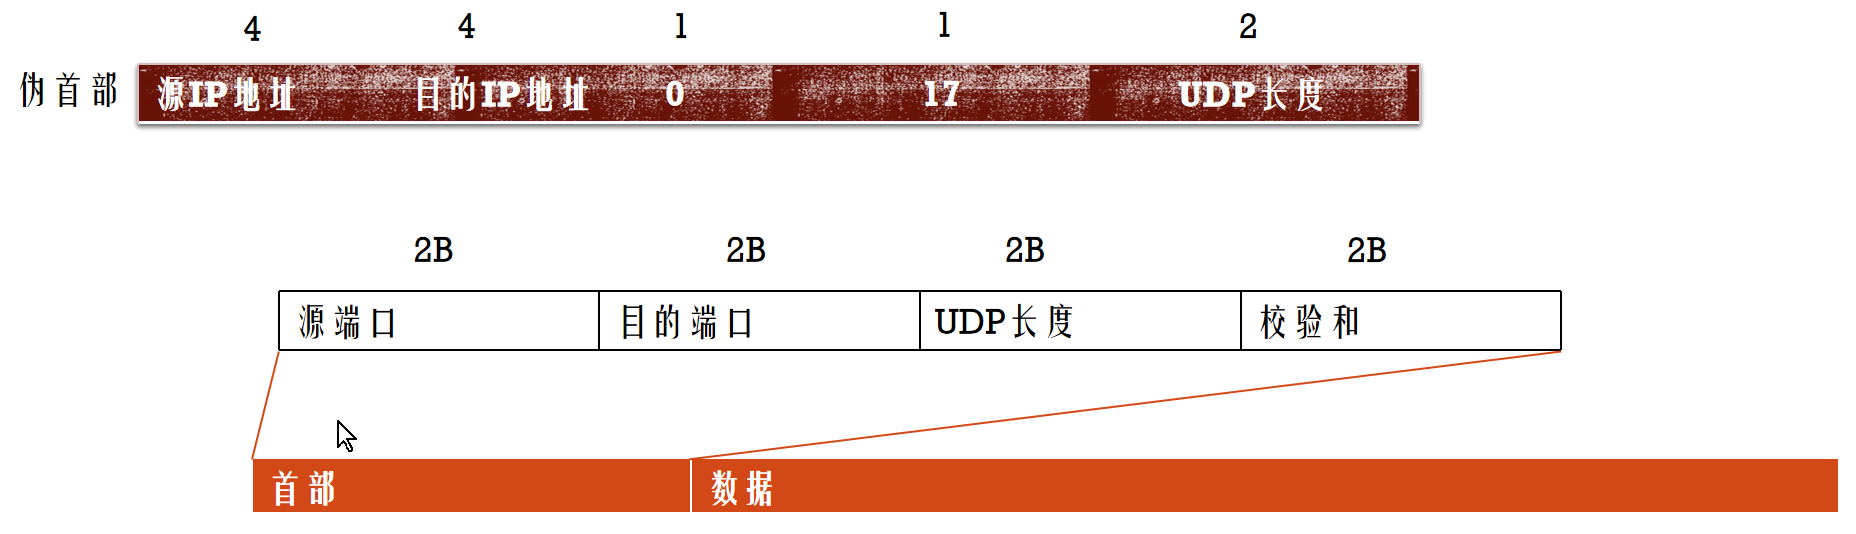
\includegraphics[width=0.65\textwidth]{lab5/udp_ip.png}
    \caption{UDP 和 IP层(网络层)之间的关系}
    \label{fig:udp_ip}
\end{figure}

可以看出,数据在传输层被封装为 UDP 数据报(包括传输层的头部信息和数据部分),最后网络层将传输层的数据进一步封装为 IP 数据报。

\subsubsection*{UDP 报文头部结构}

\begin{figure}[H]
    \centering
    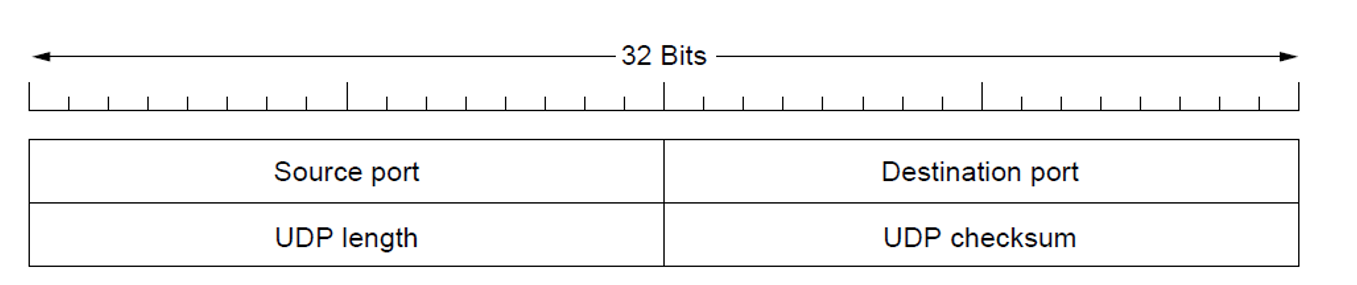
\includegraphics[width=0.6\textwidth]{lab5/udp_header.png}
    \caption{UDP 报文头部结构}
    \label{fig:udp_header}
\end{figure}


\section{实验环境}

使用 Wireshark v4.2.5, Windows 11 Pro, Wget Tools 进行实验。

实验报告使用 \LaTeX 进行撰写,使用 Vim 编辑器进行文本编辑。

\section{实验过程与分析}

\subsection{Step 1: Capture a trace}

\subsubsection{设置 Wireshark}

将过滤器设置为 udp,将混杂模式关闭,

\begin{figure} [H]
    \centering
    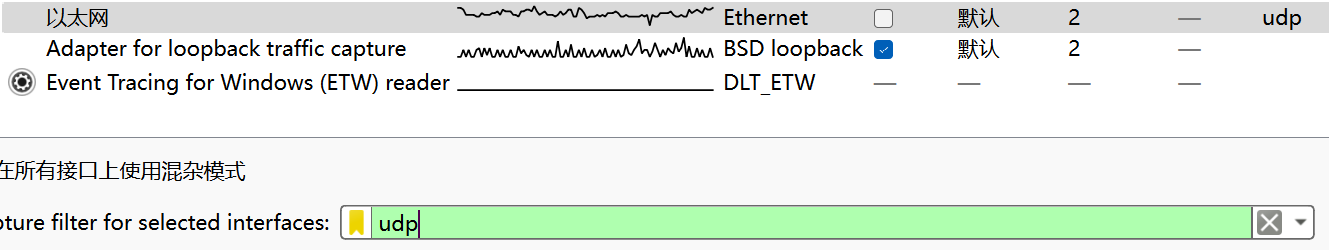
\includegraphics[width=0.7\textwidth]{lab5/udpsetting.png}
    \caption{设置 Wireshark 的过滤器}
\end{figure}

设置 rename 选项为开启,点击开始捕获。

\begin{figure}[H]
  \centering
  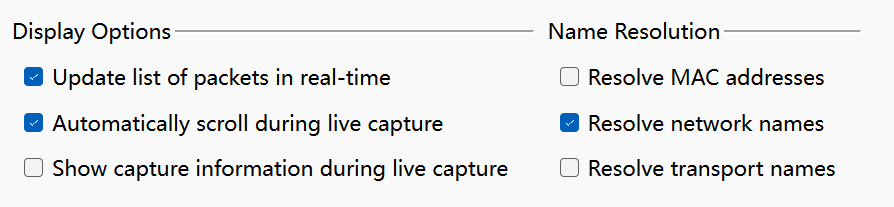
\includegraphics[width=0.5\textwidth]{lab5/rename.png}
  \caption{Wireshark Rename}
\end{figure}

\subsubsection{使用 nslookup 命令}

在命令行首先使用 \texttt{ipconfig/flushdns} 清空 DNS 缓存。

然后使用 \texttt{nslookup www.baidu.com} 命令查询域名的 DNS 服务器。

\begin{figure}[H]
    \centering
    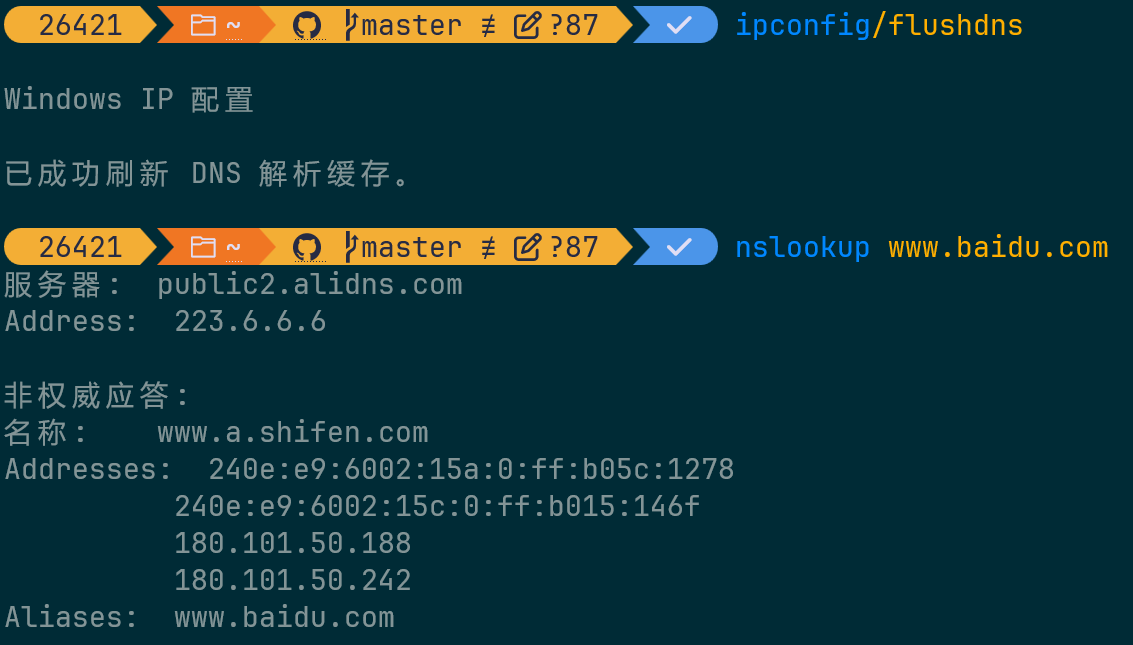
\includegraphics[width=0.5\textwidth]{lab5/nslookup.png}
    \caption{使用 nslookup 命令查询 DNS 服务器}
\end{figure}

回到 Wireshark 中,点击停止捕获,此时已经可以看到有许多刚刚捕获的 UDP 数据包。

\begin{figure}[H]
    \centering
    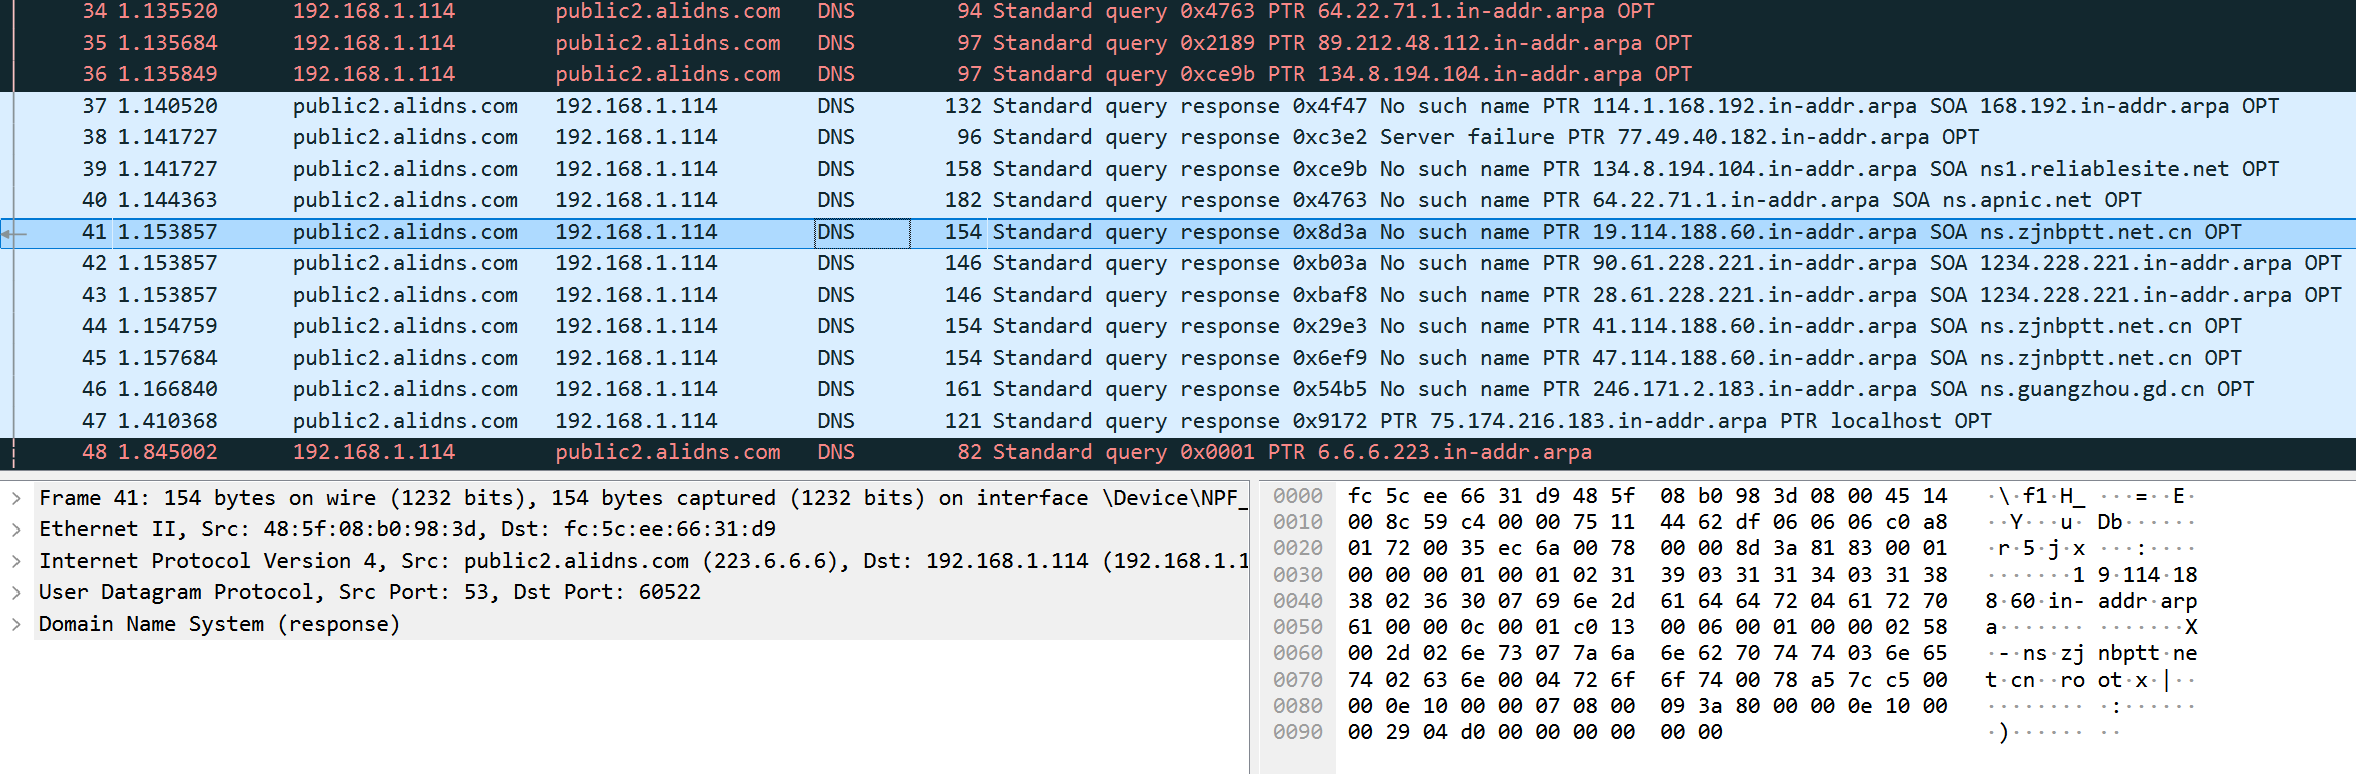
\includegraphics[width=0.8\textwidth]{lab5/dnsresult.png}
    \caption{Wireshark 捕获的 DNS 结果}
\end{figure}

\subsection{Step 2: Inspect The Trace}

可以看到在一个 UDP 信息内含有源端口、目标端口、数据长度和校验和四个部分。

\begin{figure}[H]
    \centering
    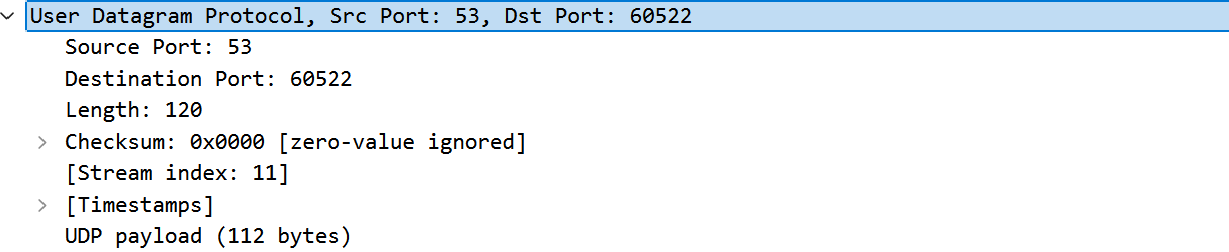
\includegraphics[width=0.65\textwidth]{lab5/udp.png}
    \caption{UDP Information}
\end{figure}

注意到此处的校验和为 \texttt{00 00},查看实验手册可以发现这里对应了一段话:

\begin{mdframed}[backgroundcolor=gray!10, linewidth=0.5pt, roundcorner=5pt]
\textit{Is your checksum carrying 0 and flagged as incorrect for UDP messages sent from your computer? On some computers, the operating system software leaves the checksum blank (zero) for the NIC to compute and fill in as the packet is sent. This is called protocol offloading.}
\end{mdframed}

\noindent 这种机制称为 \textbf{协议卸载}(Protocol Offloading),通过让网络接口卡 (NIC) 负责校验和的计算,提高了网络数据的传输性能。

\subsection{Step 3: UDP Message Structure}

根据以上捕获的信息,我们可以绘制出一个简单的 UDP 数据报的结构。

我们首先先将 Wireshark 抓包获得的数据信息进行处理,如下所示:

\begin{figure}[H]
    \centering
    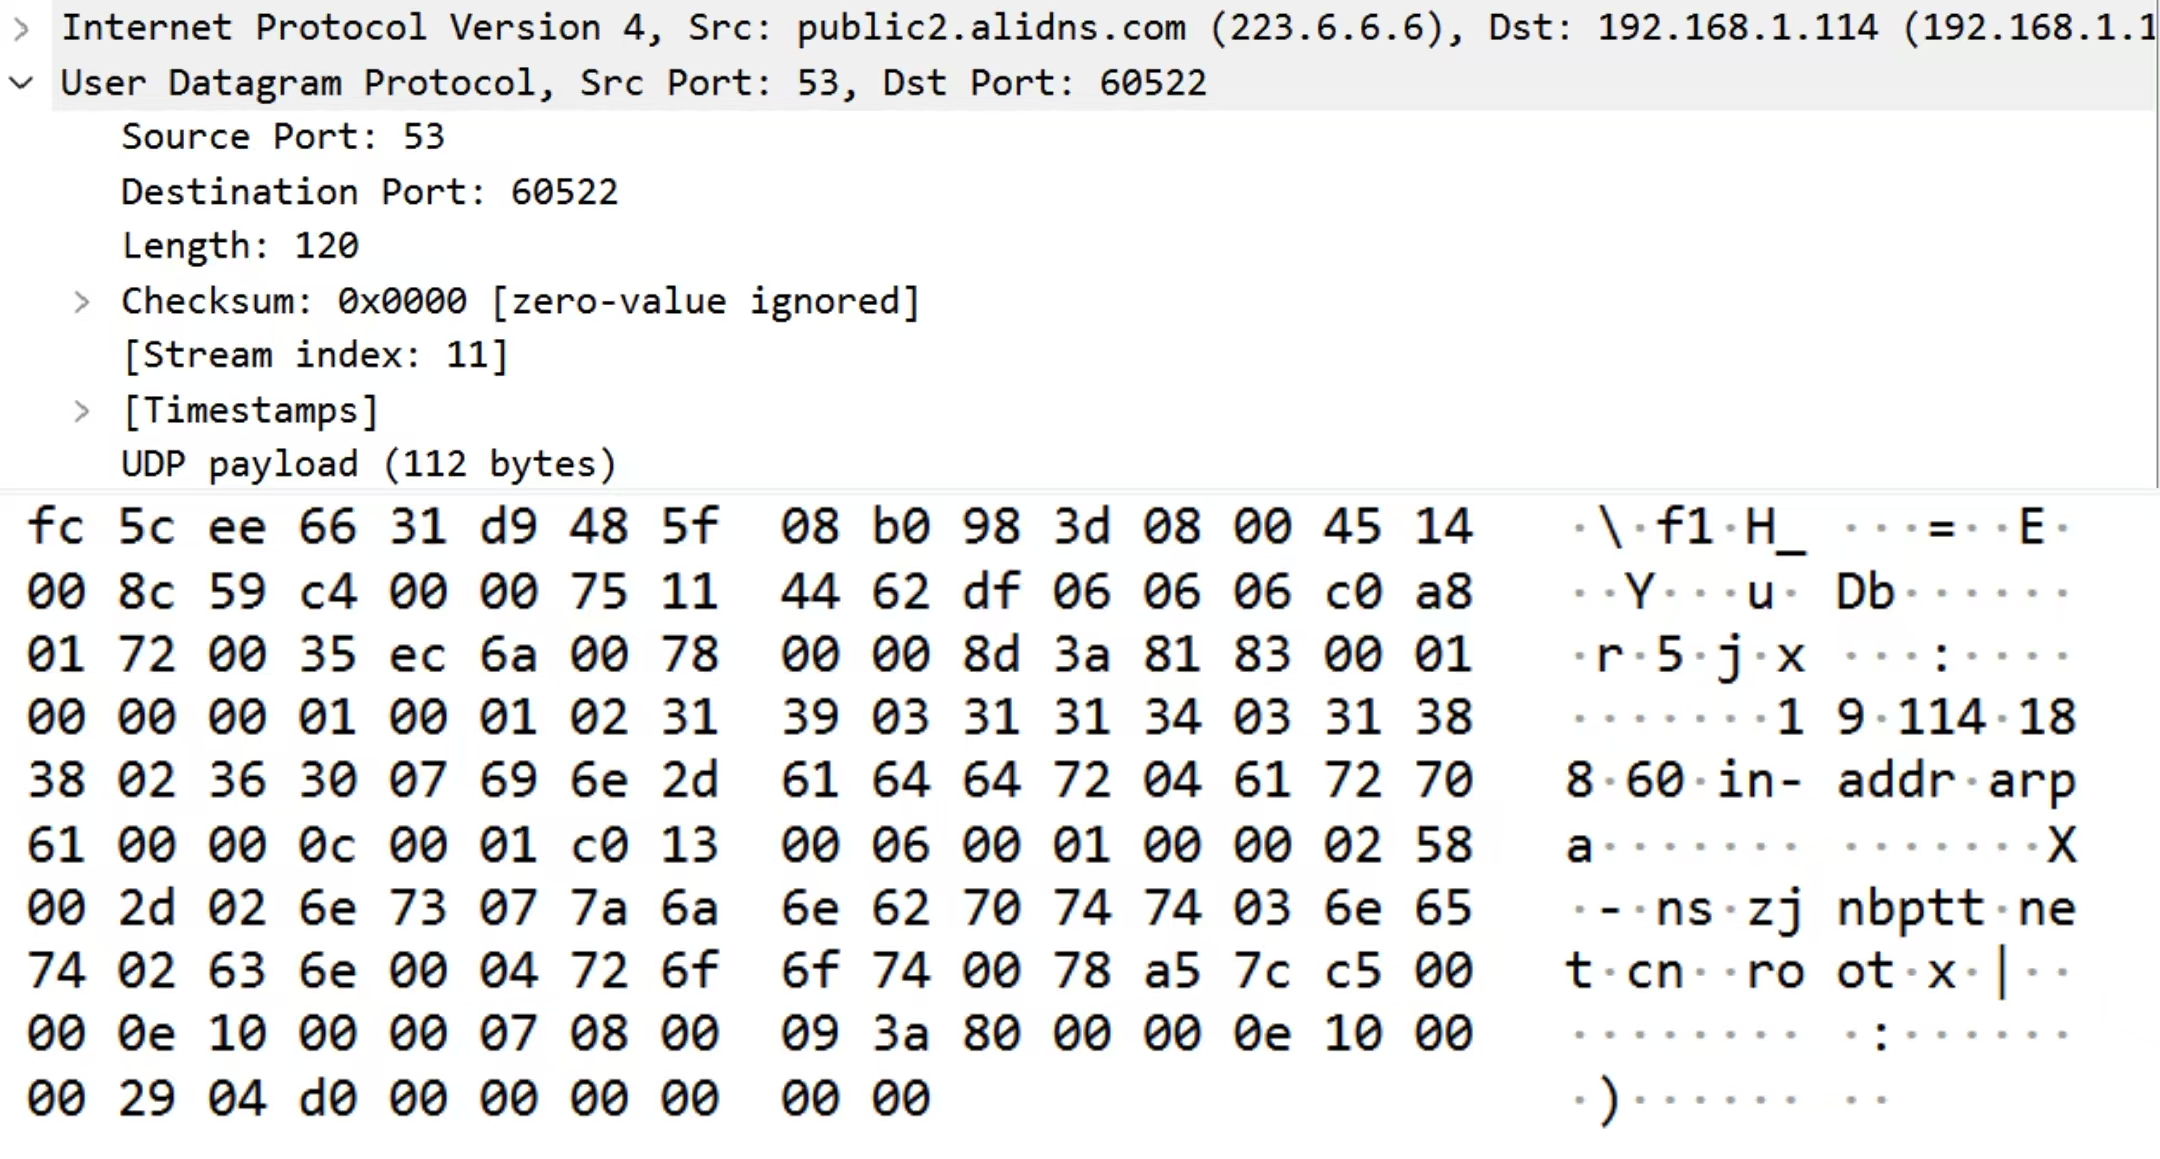
\includegraphics[width=0.6\textwidth]{lab5/combina.jpg}
    \caption{UDP 数据信息}
\end{figure}

然后我们再绘制出 UDP 数据报的结构,如下所示:

\begin{figure}[H]
    \centering
    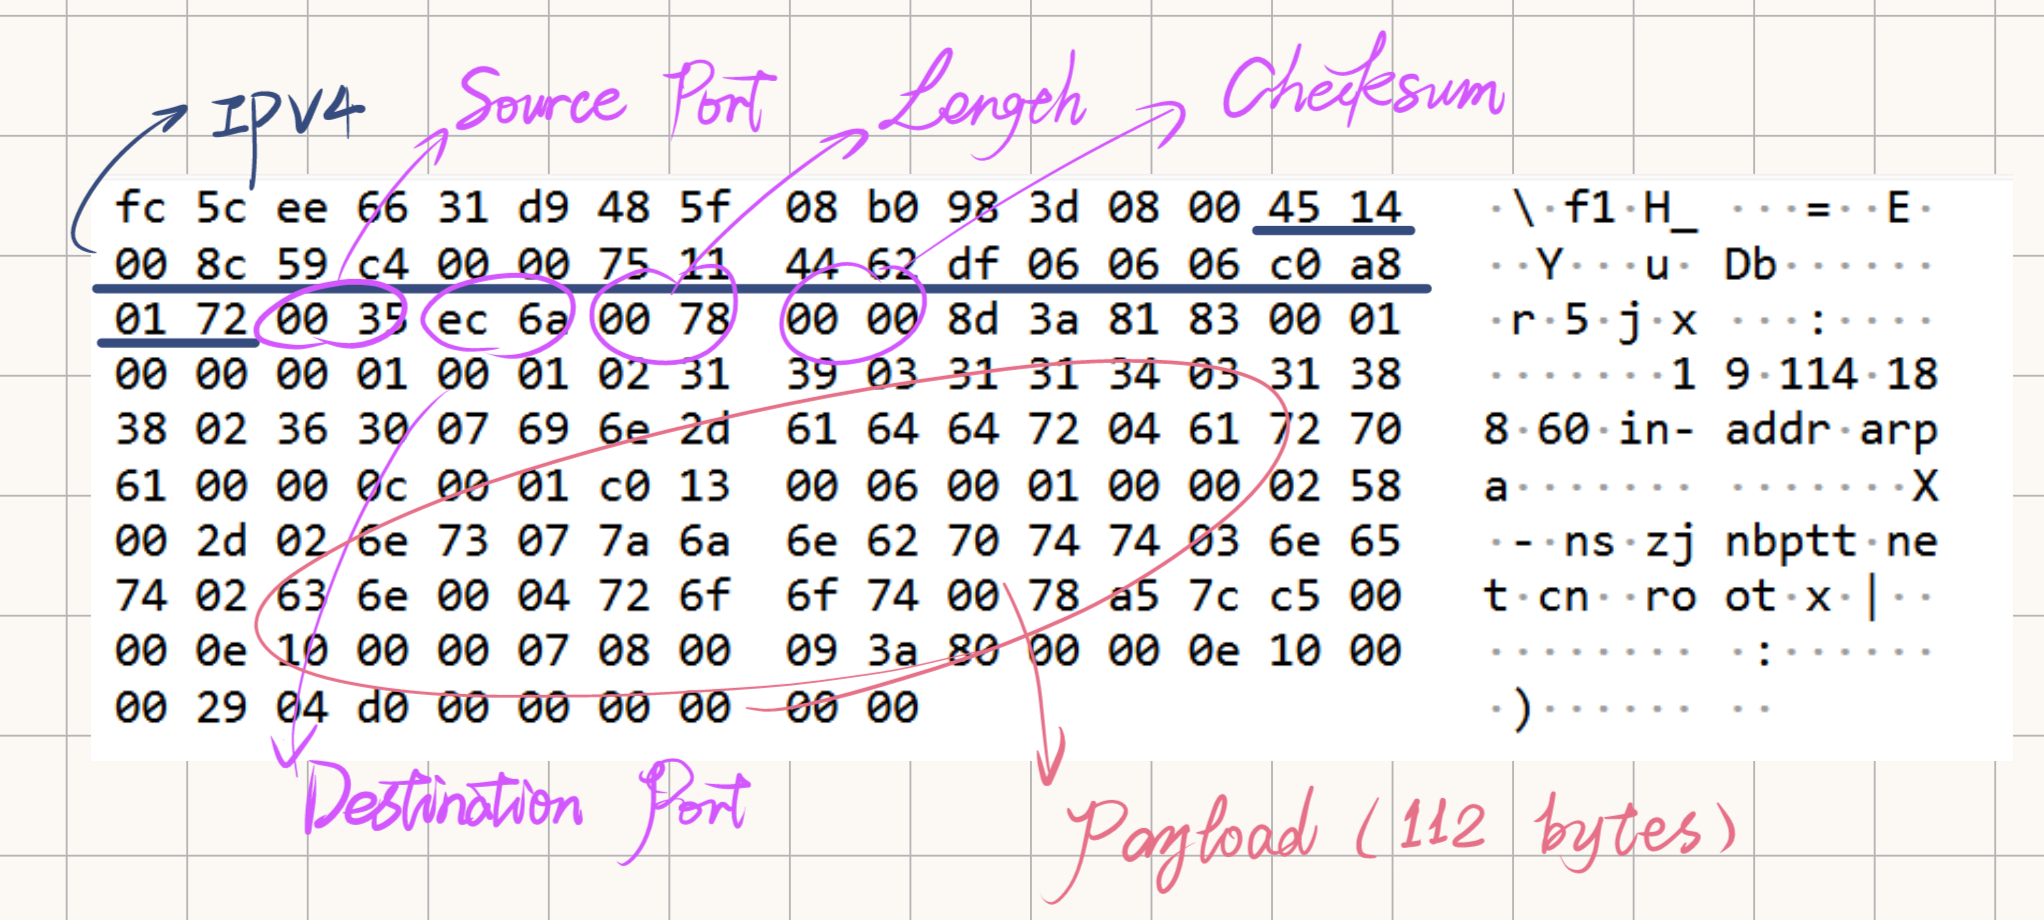
\includegraphics[width=0.65\textwidth]{lab5/draw.png}
    \caption{UDP 数据报结构}
\end{figure}

\begin{center}
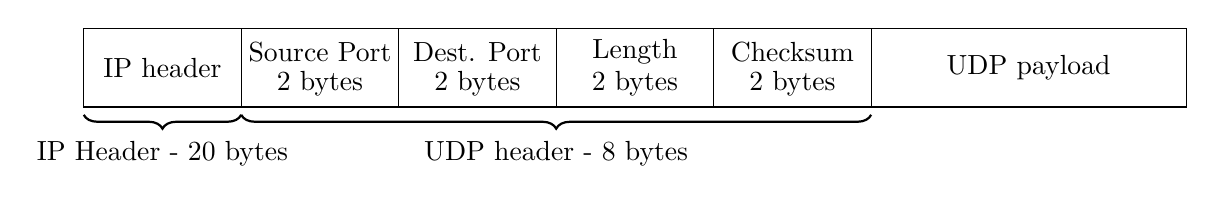
\begin{tikzpicture}[scale=1, transform shape]

% 整个框架边界
\draw (0, 0) rectangle (10, 1);

% 划分 IP Header
\draw (0, 0) -- (2, 0) -- (2, 1);
\node at (1, 0.5) {IP header};

% Source Port
\draw (2, 0) -- (4, 0) -- (4, 1);
\node at (3, 0.7) {Source Port};
\node at (3, 0.3) {2 bytes};

% Destination Port
\draw (4, 0) -- (6, 0) -- (6, 1);
\node at (5, 0.7) {Dest. Port};
\node at (5, 0.3) {2 bytes};

% Length
\draw (6, 0) -- (8, 0) -- (8, 1);
\node at (7, 0.7) {Length};
\node at (7, 0.3) {2 bytes};

% Checksum
\draw (8, 0) -- (10, 0) -- (10, 1);
\node at (9, 0.7) {Checksum};
\node at (9, 0.3) {2 bytes};

% UDP payload
\draw (10, 0) rectangle (14, 1);
\node at (12, 0.5) {UDP payload};

% UDP header description with brace
\draw [decorate, decoration={brace, amplitude=5pt, mirror}, thick] (2, -0.1) -- (10, -0.1);
\node at (6, -0.6) {UDP header - 8 bytes};

\draw [decorate, decoration={brace, amplitude=5pt, mirror}, thick] (0, -0.1) -- (2, -0.1);
\node at (1, -0.6) {IP Header - 20 bytes};

\end{tikzpicture}
\end{center}

\subsubsection{回答问题}

By looking at the details of the UDP messages in your trace, answer these questions:

\begin{ans}{问题}{问题}
\subsubsection*{问题 1}

What does the Length field include? The UDP payload, UDP payload and UDP header, or UDP payload, UDP header, and lower layer headers?

UDP数据包头中的Length字段指的是UDP有效载荷?还是UDP有效载荷加上UDP头的总长度?还是UDP有效载荷和UDP头以及低层协议的头部三者总长度?

\textbf{在 Wireshark 中很明显,Length 字段给出了:UDP 有效载荷的长度加上 UDP 报头。}

\vspace{0.5cm}

\subsubsection*{问题 2}

How long in bits is the UDP checksum? UDP头中的校验和的长度是多少位?

\textbf{16 bits long.}

\vspace{0.5cm}

\subsubsection*{问题 3}

How long in bytes is the entire UDP header? UDP头的总长度是多少字节?

\textbf{8 bites long.}
\end{ans}

\subsection{Step 4: UDP Usage}

\subsubsection{交给上一层 UDP 的字段}

IP如何知道下一个更高的协议层是UDP。答案是IP报头中有一个包含此信息的Protocol字段。

\begin{figure}[H]
    \centering
    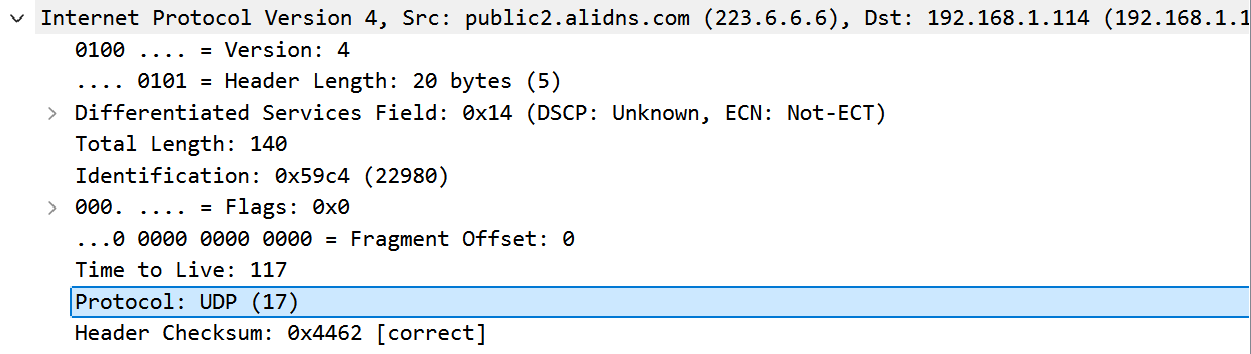
\includegraphics[width=0.7\textwidth]{lab5/ip.png}
    \caption{IP Header}
\end{figure}

此处,代表 UDP 协议的值为 17。

\subsubsection{其他类型的 UDP 包}

在实验手册中有提到:

\begin{mdframed}[backgroundcolor=gray!10, linewidth=0.8pt, roundcorner=5pt]
    \textit{You can see this by sorting on the Source and Destination columns. The source and destinations will be domain names, if Network layer name resolution is turned, and otherwise IP addresses.}
\end{mdframed}

我们可以先使用 \texttt{ipconfig} 命令来读取本机计算机的地址,然后去查看 MDNS(使用 IP 多播的 DNS 流量)包,这是一个经典的满足上述情况的协议。

\begin{figure}[H]
    \centering
    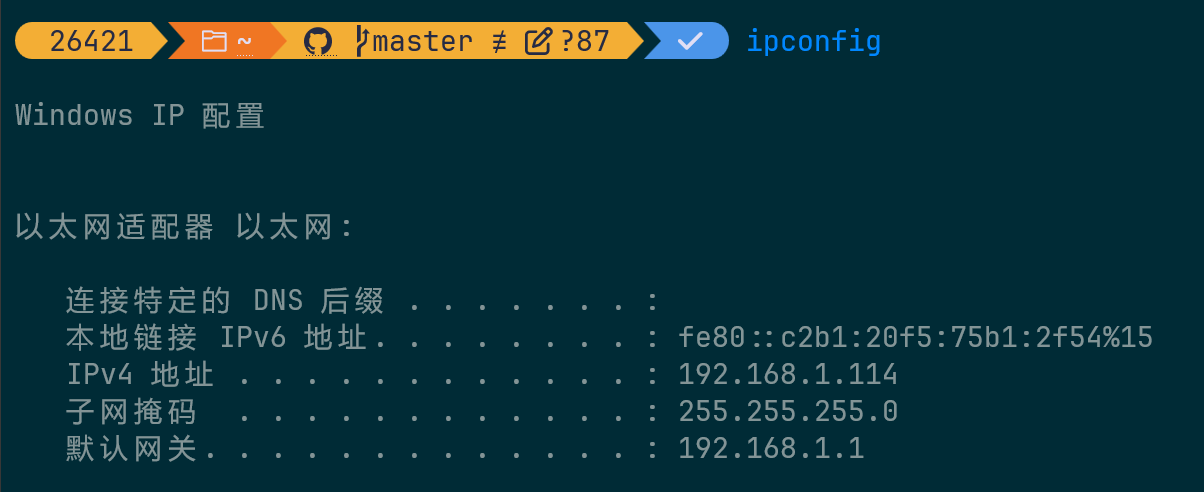
\includegraphics[width=0.5\textwidth]{lab5/ipconfig.png}
    \caption{ipconfig}
\end{figure}

MDNS 协议的发送地址和目标地址都不是本地计算机。

它将主机名解析为不包含本地名称服务器的小型网络中的 IP 地址。

\begin{figure}[H]
    \centering
    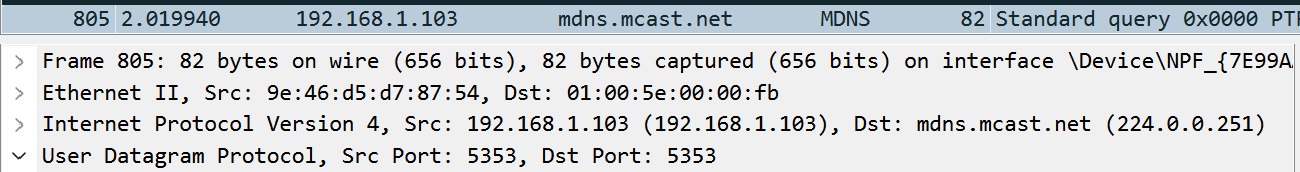
\includegraphics[width=0.8\textwidth]{lab5/mdns.png}
    \caption{MDNS}
\end{figure}

该数据包的 Destination 地址为:\textbf{224.0.0.251},查阅资料(\href{https://blog.csdn.net/m0_51551385/article/details/122327966}{计算机网络——组播地址(多播地址、D类地址)详解})发现,\textbf{224.0.xx.xx} 的地址均用于 mDNS 协议。

\subsubsection{一般 UDP 消息的长度}

查看 Wireshark 中获取的 Length 字段,可以发现 UDP 数据包的长度大多数情况下都在 100 字节左右,最小的有 50 字节,最大的达到了 182 字节。

\begin{figure}[H]
    \centering
    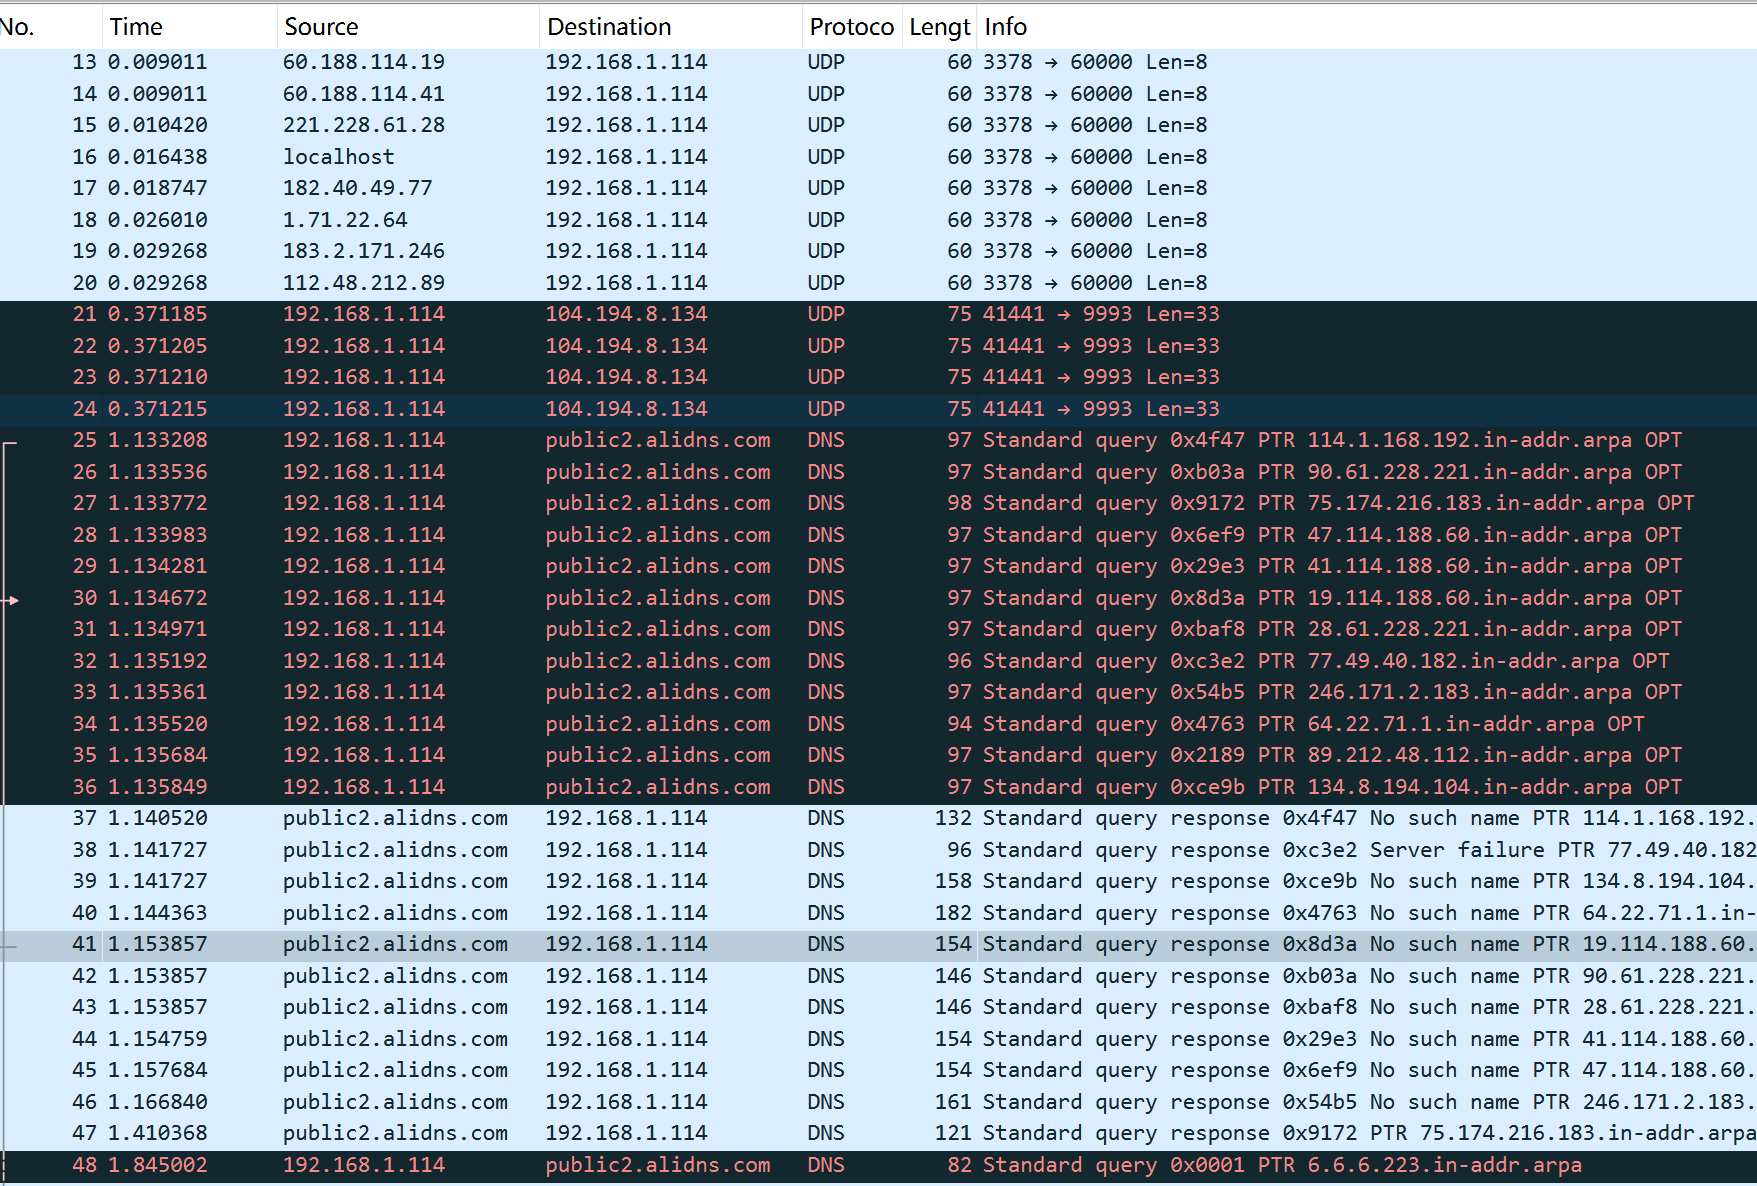
\includegraphics[width=0.8\textwidth]{lab5/length.png}
    \caption{UDP 数据包长度}
\end{figure}

显然,在我捕获的 Trace 中,基本上 Typical Length 即为 100 字节左右。

\subsection{Explore on your own}

\begin{mdframed}[backgroundcolor=gray!10, linewidth=0.8pt, roundcorner=5pt]
    \textit{We encourage you to keep exploring on your own, but there is not much more to UDP. Instead, you might examine the traffic of UDP-based applications to look at packet sizes and loss rates. Voice-over-IP and its companion protocols like RTP (Real-Time Protocol) are good candidates. Similarly, you might explore streaming and real-time applications to see which use UDP and which use TCP as a transport.}
\end{mdframed}

\subsubsection{基于 UDP 的应用流量}

我们可以使用 VLC 等媒体播放器来观察 UDP 协议的应用流量。

参考链接:\href{https://blog.csdn.net/u014696856/article/details/126341960?spm=1001.2101.3001.6661.1&utm_medium=distribute.pc_relevant_t0.none-task-blog-2%7Edefault%7EBlogCommendFromBaidu%7ERate-1-126341960-blog-128813090.235%5Ev43%5Epc_blog_bottom_relevance_base9&depth_1-utm_source=distribute.pc_relevant_t0.none-task-blog-2%7Edefault%7EBlogCommendFromBaidu%7ERate-1-126341960-blog-128813090.235%5Ev43%5Epc_blog_bottom_relevance_base9&utm_relevant_index=1}{\underline{RTSP流媒体测试地址}}

在注册了免费的 RTSP 流 url 后,我们首先在 VLC 流媒体播放器中播放:

\begin{figure}[H]
    \centering
    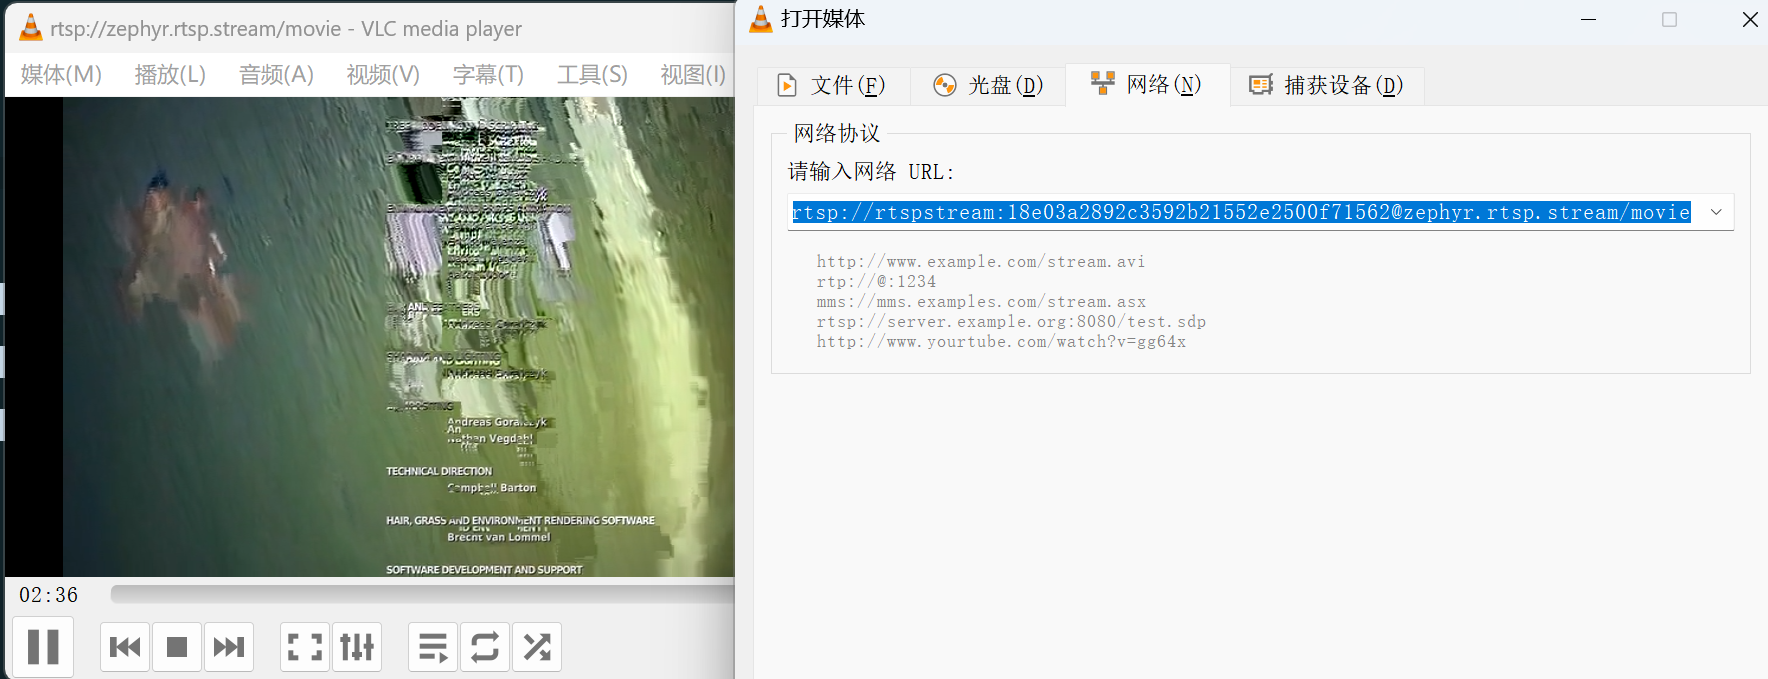
\includegraphics[width=0.65\textwidth]{lab5/url.png}
    \caption{VLC 流媒体播放器}
\end{figure}

之后我们在 Wireshark 中开始捕获,并且把过滤器设置为 udp,右键一个 udp 协议包,选择 Decode As,在弹出的窗口中,
将当前协议修改为 RTP,点击 OK,Wireshark 便会将这些 UDP 数据包重新解码为 RTP 数据包。

之后在工具栏中,进入 RTP 流分析,点击分析,便能够实时读取 RTP 流,效果如下:

\begin{figure}[H]
    \centering
    % 第一张子图
    \begin{subfigure}[b]{0.25\textwidth}
        \centering
        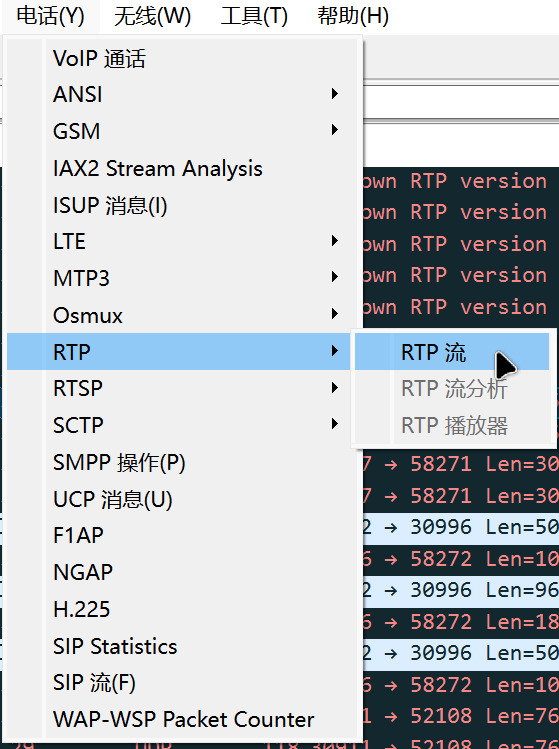
\includegraphics[width=\textwidth]{lab5/tele.png}
        \caption{Decode As}
    \end{subfigure}
    \hspace{0.1\textwidth}
    % 第二张子图
    \begin{subfigure}[b]{0.45\textwidth}
        \centering
        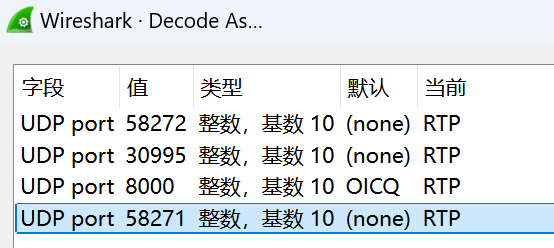
\includegraphics[width=\textwidth]{lab5/UDP2RTP.png}
        \caption{进入 RTP 流分析}
    \end{subfigure}

    \caption{设置从 UDP 协议解码至 RTP 协议}
    \label{fig:rtp_example}
\end{figure}

\begin{figure}[H]
    \centering
    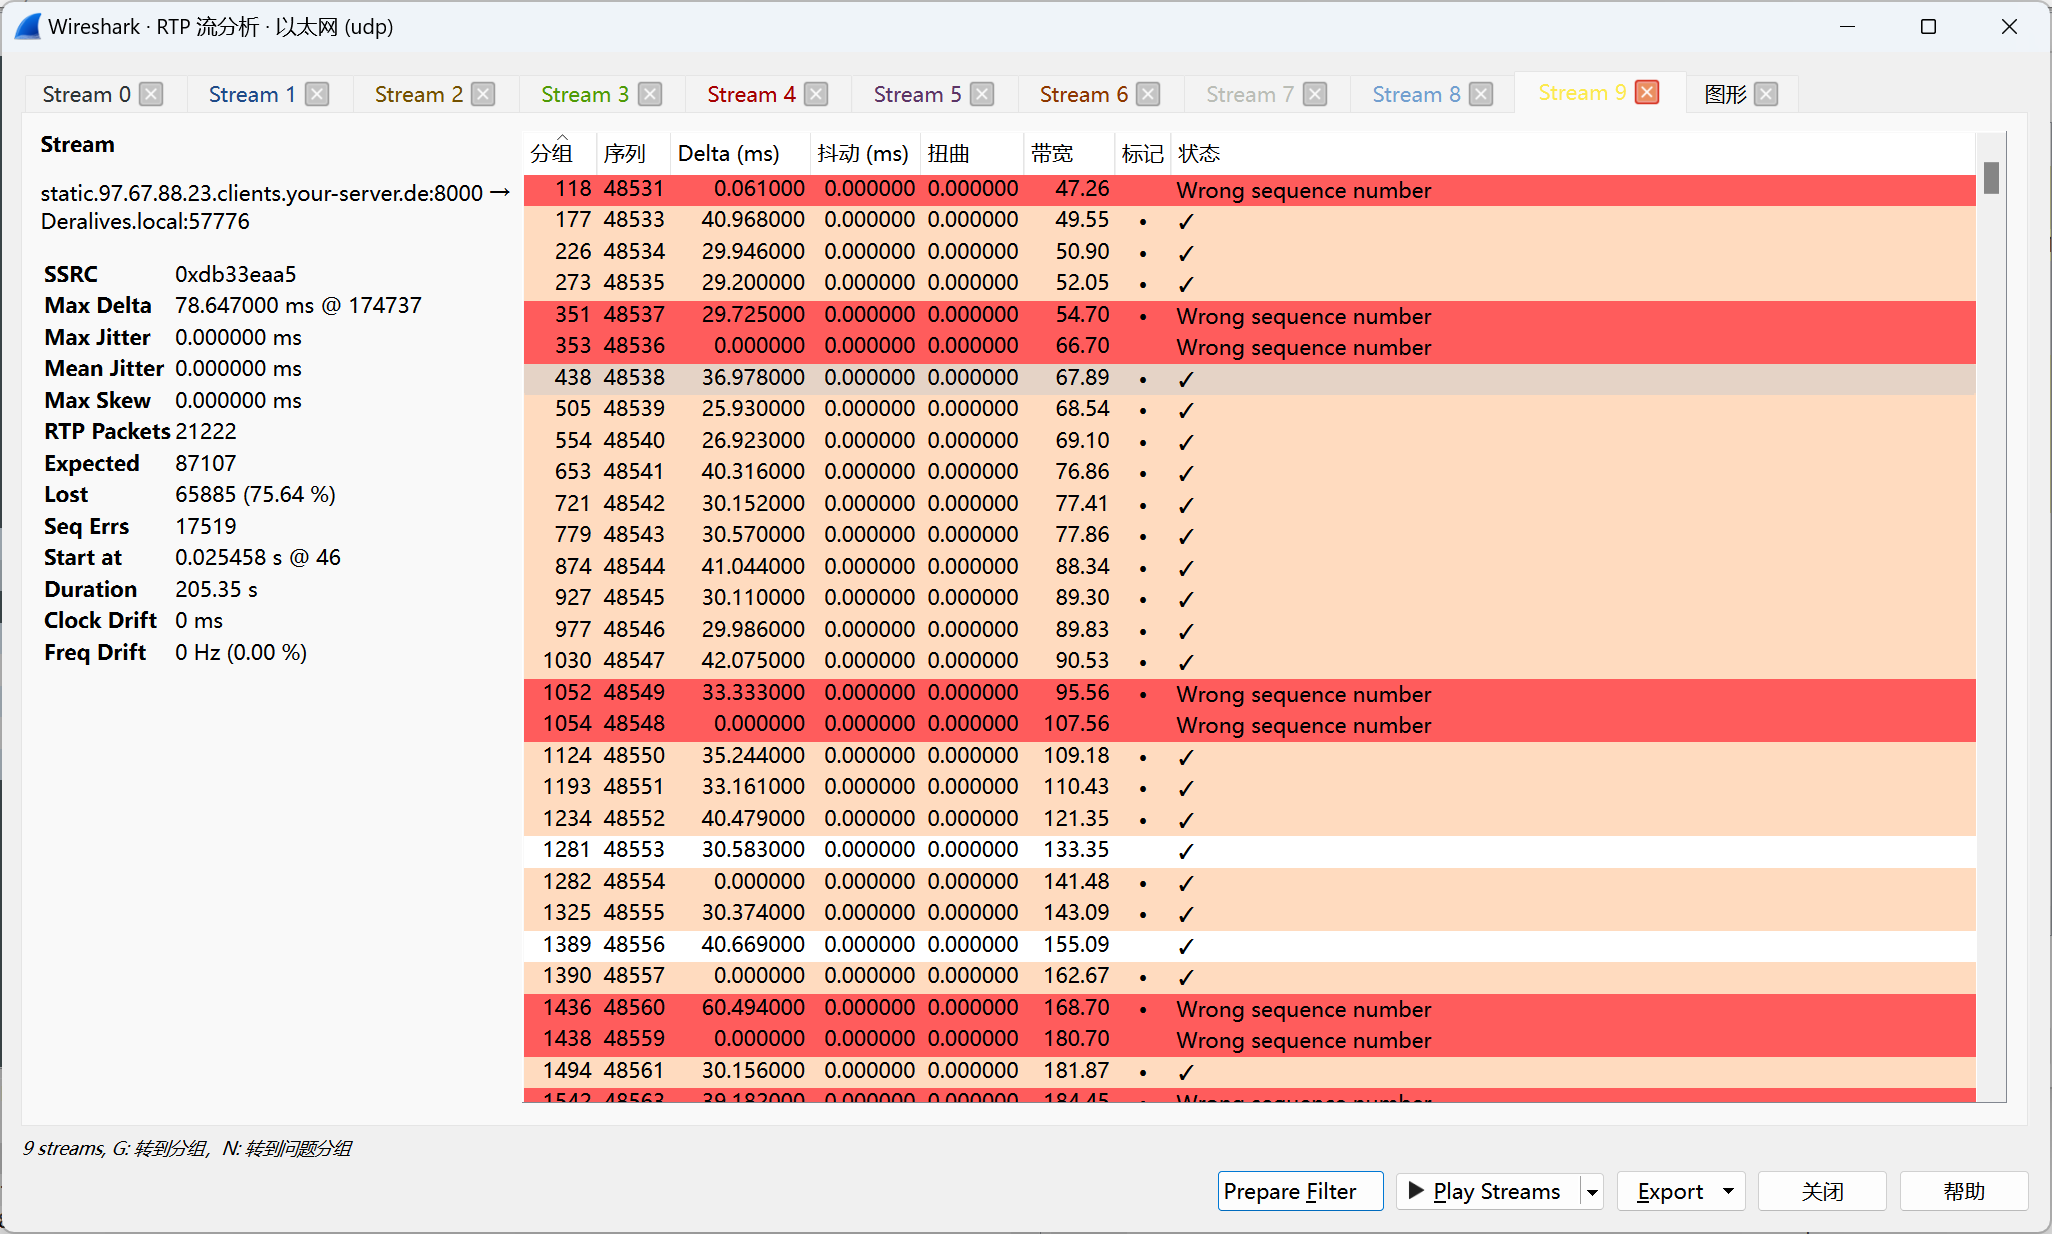
\includegraphics[width=0.65\textwidth]{lab5/Analysis.png}
    \caption{RTP Analysis}
\end{figure}

在这里的 Stream 9 中,我们可以看到左边数据丢包率很高。达到了 75.64\%。

所以在该端口的流传输丢包率较高,我们通过观看视频画面也可以发现有所扭曲:

而带宽方面,可以反映数据包的大小,当然我们也可以通过在 Wireshark 的主界面查看解析成为 RTP 协议后的包的 Length 字段大小。

\begin{figure}[H]
    \centering
    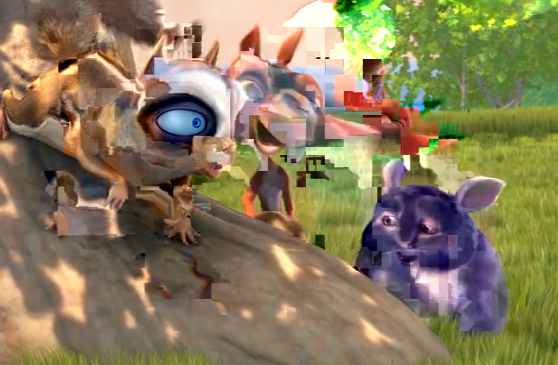
\includegraphics[width=0.3\textwidth]{lab5/6.png}
    \caption{丢包率较高的视频}
\end{figure}

\subsubsection{探索流和实时应用程序}

\subsection*{TCP(传输控制协议)}
TCP 是一种面向连接的、可靠的传输协议,主要应用于对数据准确性要求高的场景。它会确保数据的完整性,即使速度相对较慢,也能够保证数据准确无误。以下是 TCP 常见的应用场景:
\begin{itemize}
    \item \textbf{文件传输}:如 FTP 和 HTTP 协议。这些场景对数据的完整性要求非常高,即使速度稍慢,也要确保每一个字节的数据都能正确传输。
    \item \textbf{电子邮件服务}:包括 POP3、IMAP 和 SMTP 协议。邮件传输不需要实时性,但数据必须准确无误,以保证完整的邮件内容和附件发送。
\end{itemize}

\subsection*{UDP(用户数据报协议)}
UDP 是一种无连接的、不可靠的传输协议,适用于对速度和实时性要求高,但对偶尔丢包容忍度较高的场景。以下是 UDP 的常见应用:
\begin{itemize}
    \item \textbf{即时通信}:例如 QQ 聊天等应用。虽然偶尔丢失一个数据包不会影响整体交流,但传输速度要快,以确保消息及时送达。
    \item \textbf{在线视频流媒体}:如 RTSP 协议,主要用于视频播放。视频传输更强调流畅度和实时性,即使偶尔丢失一帧图像,也不会严重影响用户体验。
    \item \textbf{网络语音通话}:如 VoIP(网络电话)。语音数据包通常较小,传输过程中即使偶尔出现断音或失真,用户也能接受,而快速传输是关键。
\end{itemize}

\subsection*{使用 Moonlight 进行串流时的 UDP 协议}

\textbf{串流游戏服务(Moonlight)}:Moonlight 是基于 \textbf{NVIDIA GameStream} 协议的游戏串流工具,它利用 UDP 实现低延迟的数据传输。对于游戏串流而言,实时性和流畅度至关重要,哪怕偶尔有轻微丢包,也不影响整体游戏体验。通过 UDP,高速传输图像和输入数据,确保玩家能够远程进行低延迟、高帧率的游戏操作。

在我的工作流中,我在寝室内便是使用 Moonlight 进行串流,使得第二台电脑能够成为我的副屏,这一切实际上就是 Moonlight 进行传输的。

以下是我使用 UDP 抓包时的结果,此时我正在编写本实验报告,使用平板电脑串流成为第二屏幕:

\begin{figure}[H]
    \centering
    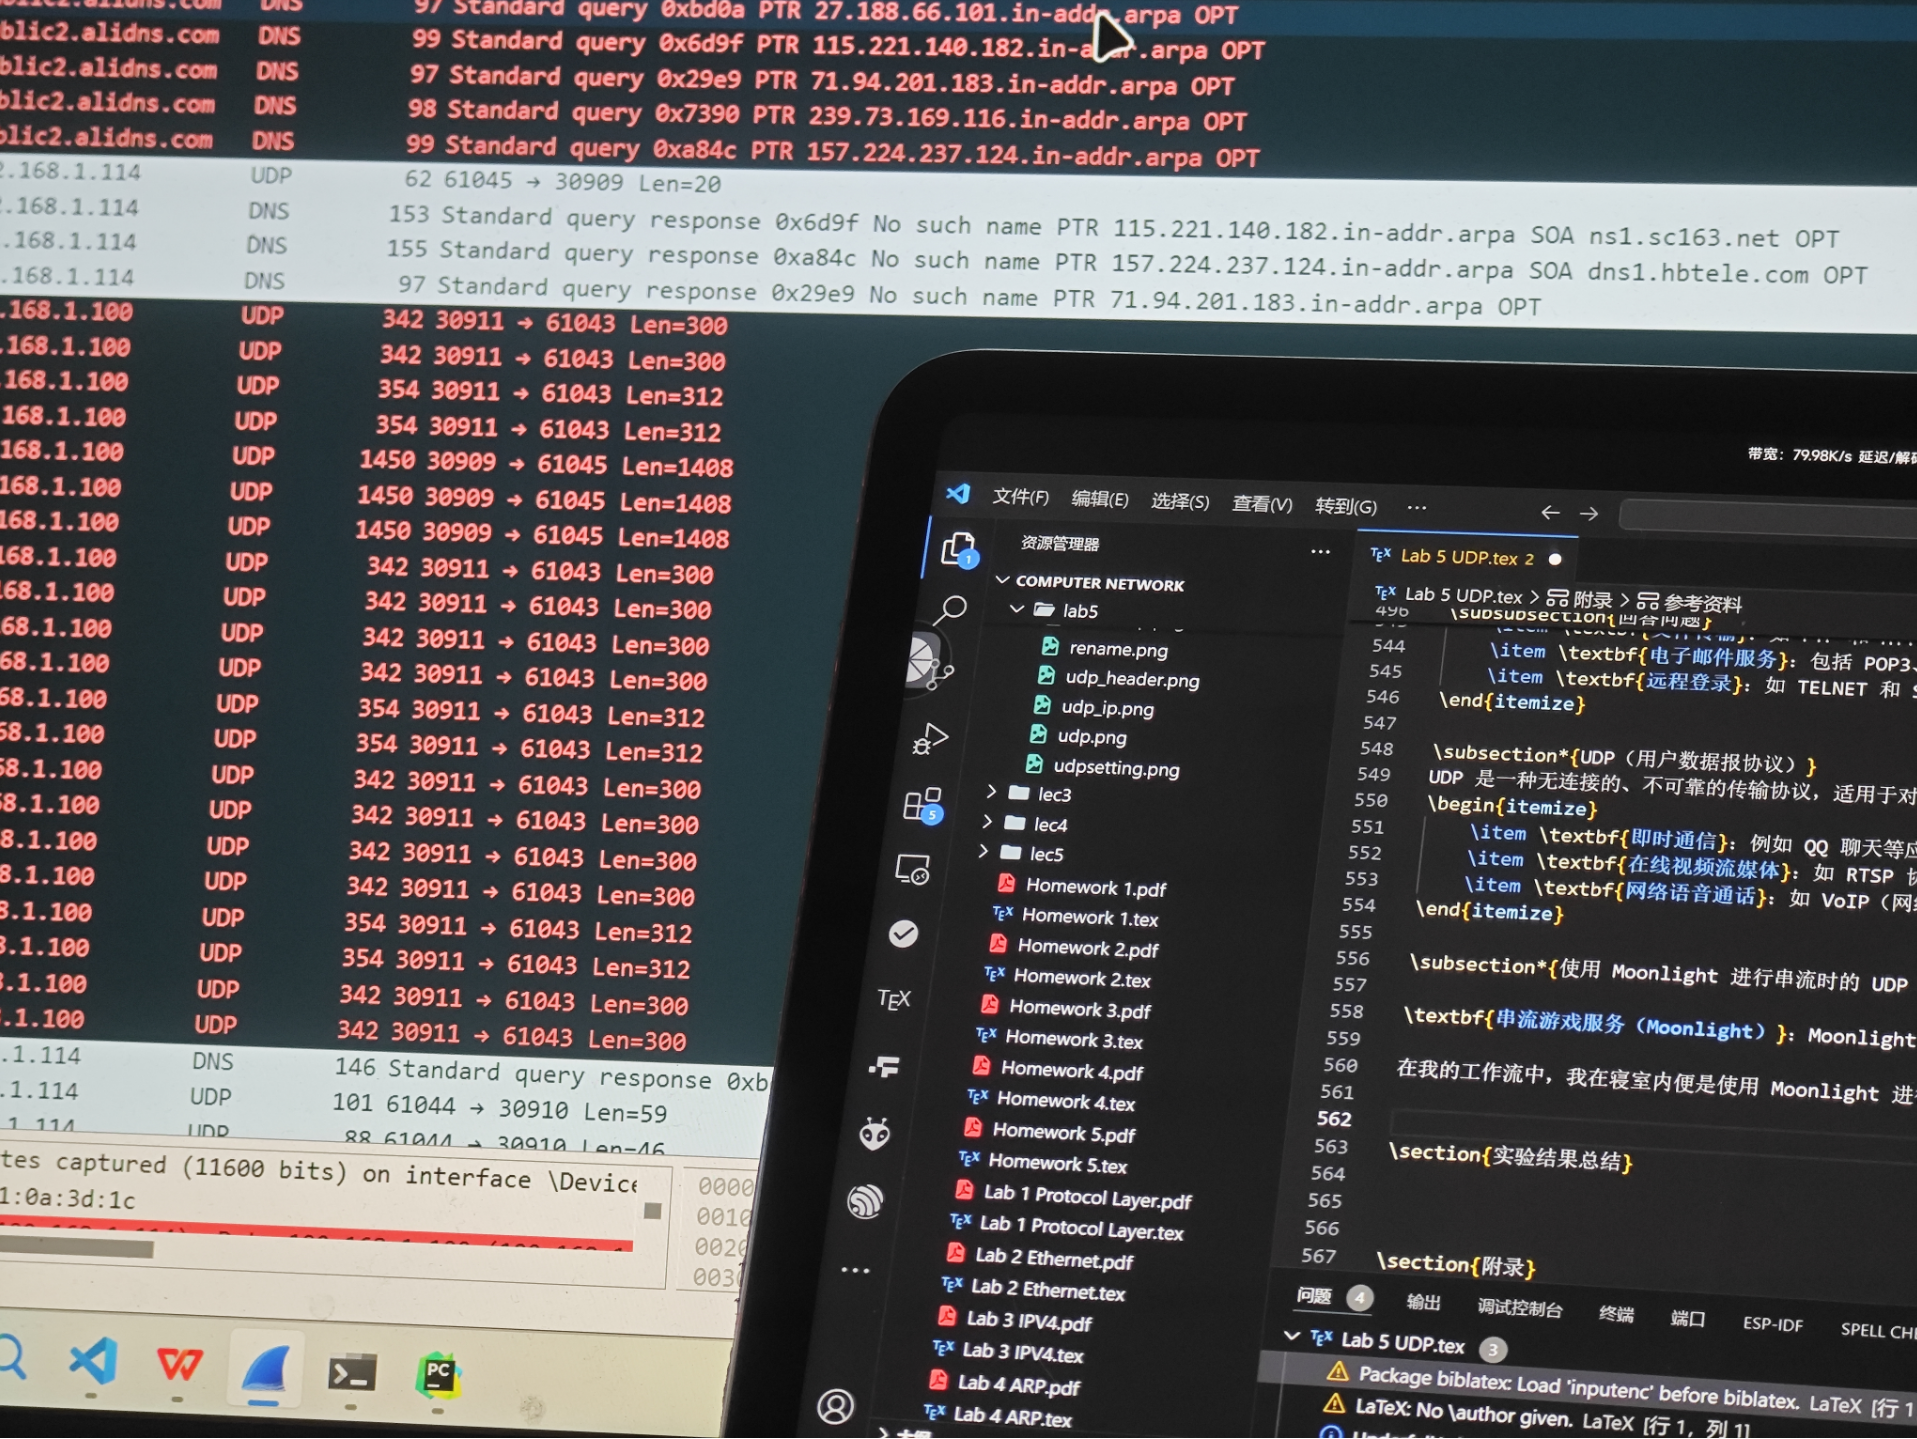
\includegraphics[width=0.6\textwidth]{lab5/pad.png}
    \caption{Moonlight 串流时 UDP 协议}
\end{figure}

打开 Sunshine 的网络设置选项,可以看到此时 UDP 30911 端口正在进行数据传输。

这就是实时把数据传输到了我的平板之上:

\begin{figure}[H]
    \centering
    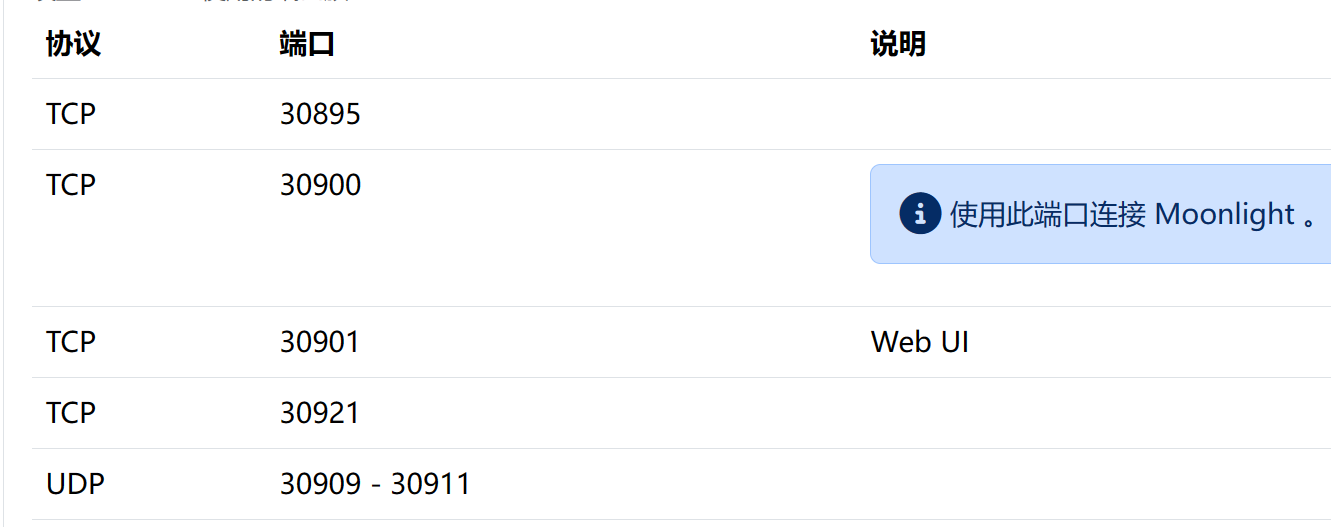
\includegraphics[width=0.65\textwidth]{lab5/moonlight.png}
    \caption{Sunshine 网络设置}
\end{figure}

\section{实验结果总结}


通过本次实验,我掌握了如何使用 \textbf{Wireshark} 工具捕获 \textbf{UDP} 数据包,并对 \textbf{UDP 协议} 有了更深入的理解。我学会了分析 UDP 协议头的各个字段,理解了它们的具体含义,以及整个 UDP 协议头固定为 \textbf{8 字节} 的长度。

此外,通过观察不同基于 UDP 传输的协议内容,我进一步了解了 \textbf{UDP 的适用场景和领域}。同时,在进行相关知识扩展时,我接触到了此前未曾了解的网络协议,例如:
\begin{itemize}
    \item \textbf{mDNS}(多播 DNS):用于局域网内的设备名称解析和发现;
    \item \textbf{NBNS}(NetBIOS 名称服务):提供局域网设备名称解析服务;
    \item \textbf{SSDP}(简单服务发现协议):用于设备和服务的发现与广播。
\end{itemize}

这些协议在局域网中的设备发现、名称解析等方面发挥了重要作用。这次实验不仅帮助我巩固了 UDP 的基础知识,也拓展了我的网络协议视野。

\section{附录}

\subsection*{参考资料}

\begin{itemize}
    \item 计算机网络——组播地址(多播地址、D类地址)详解:\href{https://blog.csdn.net/m0_51551385/article/details/122327966}{\underline{https://blog.csdn.net/m0\_51551385/article/details/122327966}}
    \item VLC:\href{https://www.videolan.org/}{\underline{https://www.videolan.org/}}
    \item RTSP 流媒体测试地址:\href{https://rtsp.stream/}{\underline{https://rtsp.stream/}}
\end{itemize}

\end{document}